
\section{Durchführung}
\label{sec:Durchführung}

\subsection{Messvorgang zur Bestimmung des Winkels $\phi$ zwischen den brechenden Oberflächen des Prismas}

Zur Bestimmung des Winkels $\phi$ zwischen den brechenden Oberflächen des Prismas wird das Prisma mit seiner brechenden Kante auf das Kollimatorrohr ausgerichtet. Unter den Winkeln $\phi_.l$ und $\phi_.r$ werden mit dem Fernrohr die reflektierten Stahlen wie in Abbildung \ref{fig:phiMessung} zu sehen ausgemessen. Aus $\phi_.l$ und $\phi_.r$ wird $\phi$ bestimmt durch:
\begin{equation}
\phi = \frac{\phi_r -\phi_l}{2} \label{eq:phi}
\end{equation} 
Die Messung wird mehrmals unter leicht unterschiedlicher Ausrichtung des Glasprismas wiederholt und der Mittelwert von $\phi$ wird gebildet.
 
\begin{figure}
\centering
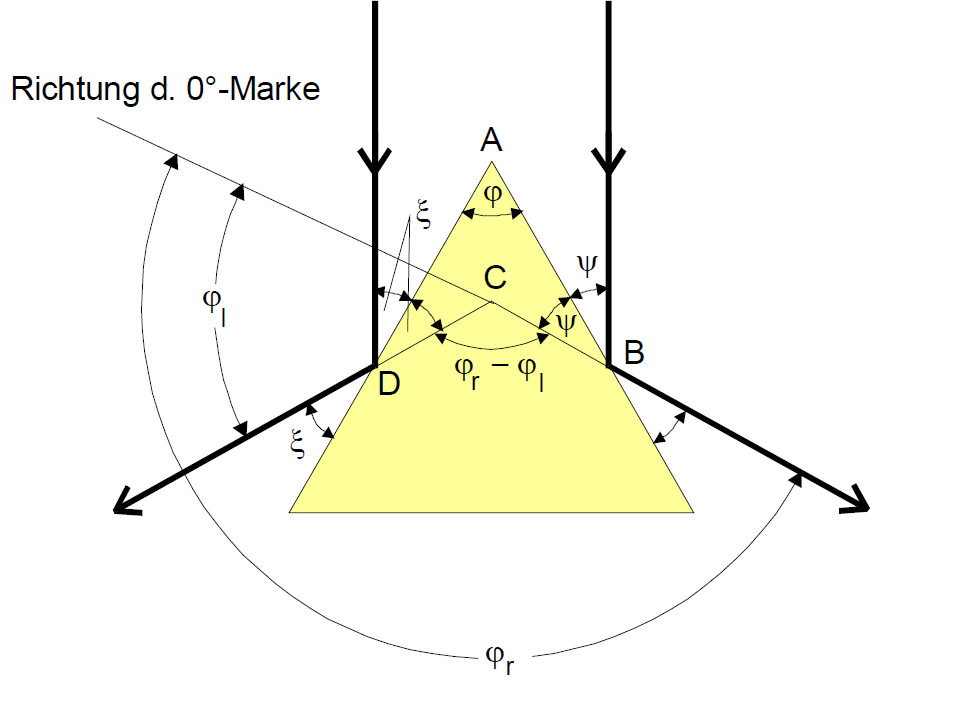
\includegraphics[width=\linewidth-50pt,height=\textheight-50pt,keepaspectratio]{content/images/phiMessung.png}
\caption{Schematische Skizze zur Bestimmung des Winkels $\phi$ \cite{V402}.}
\label{fig:phiMessung}
\end{figure}

\subsection{Messvorgang zur Bestimmung der Brechungswinkel $\eta_i$ für die Spektrallinien einer Quecksilber-Cadmium Lampe}

Zur Bestimmung der Brechungswinkel $\eta_i$ für die Spektrallinien der Quecksilber-Cadmium Lampe wird das Prisma wie in Abbildung \ref{fig:etaMessung} zu sehen mit einer der brechenden Kanten auf das Kollimatorrohr ausgerichtet. Das Prisma wird dabei so ausgerichtet, dass das Spaltbild des gebrochenen Strahlenbündels mit dem des reflektierten Strahlenbündels zusammenfällt. Mit dem Fernrohr werden die Winkel $\Omega_.{l_i}$ für die verschiedenen Spektrallinien bestimmt, wobei auf die korrekte Ausrichtung des Fadenkreuzes zu achten ist. Für die Messung der $\Omega_.{r_i}$ wird die Messung mit einer Spiegelsymmetrischen Stellung des Prismas wiederholt. Aus den $\Omega_.{l_i}$ und $\Omega_.{r_i}$ werden die $\eta_i$ bestimmt nach:
\begin{equation}
\eta_i = 180\si{grad}-(\Omega_.{r_i}-\Omega_.{l_i}) \label{eq:eta}
\end{equation} 

\begin{figure}
\centering
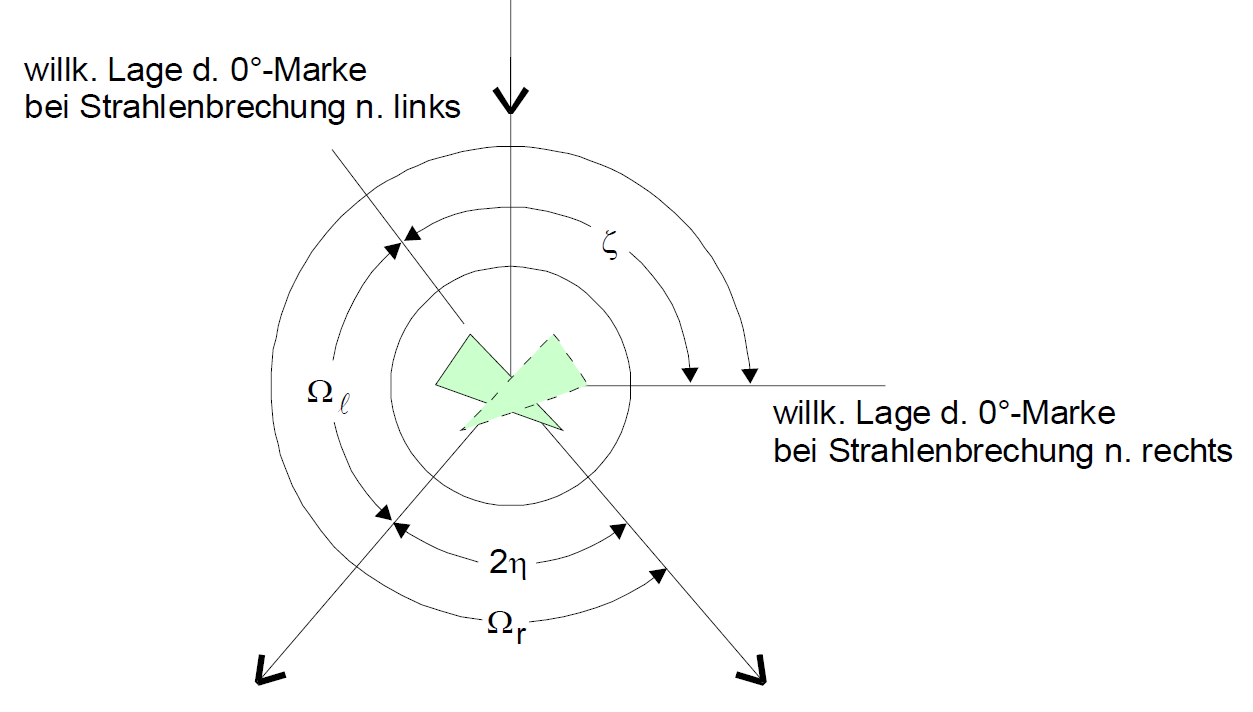
\includegraphics[width=\linewidth-50pt,height=\textheight-50pt,keepaspectratio]{content/images/etaMessung.png}
\caption{Schematische Skizze zur Bestimmung des Winkels $\eta$ \cite{V402}.}
\label{fig:etaMessung}
\end{figure}

%\subsection{Bestimmung der Dispersionskurve, der Abelschen Zahl des Glasmaterials, dem Auflösungsvermögen des Prismenspektralapparates und der zum sichtbaren Spektralbereich nächsten Absorptionsstelle}
%
%Es werden die Brechungsindizes in Abhängigkeit von den Wellenlängen berechnet.
%Aus den erhaltenden Werten wird die Dispersionskurve und die Abweichung der Werte von der Kurve bestimmt. Mithilfe der Dispersionsgleichung wird die Abelsche Zahl für das Material des Glasprismas, sowie das theoretische Auflösungsvermögen des Prismenspektralapparates für die Wellenlängen $\lambda_.C$ und $\lambda_.F$ der Fraunhoferschen Linien berechnet. Dabei wird angenommen, dass das Prisma voll ausgeleuchtet ist. Aus den optimierten Parametern der bestimmten Dispersionsgleichung wird die dem Spektralbereich am nächsten gelegene Absorptionsstelle berechnet. 
 